\chapter{SQL - Structured Query Language}
SQL è un linguaggio per la definizione e la manipolazione dei dati
in database relazionali adottato da molti DBMS. \\
Ci sono diverse versioni, la prima versione ufficiale risale al 1986.
Poi sono state rilasciate altre versioni come SQL-89, SQL-2, SQL-3\dots\\
Noi faremo riferimento principalmente a SQL-2. Questa versione è ricca e complessa,
tanto che nessun sistema commerciale lo implementa in maniera completa.\\
Esistono 3 livelli di conformità:
\begin{itemize}
  \item Entry level: molto simile a SQL-89
  \item Intermediate level: versione che soddisfa le esigenze di mercato
  \item Full level: versione completa anche delle funzioni avanzate che non sono realizzate
        in alcun DBMS
\end{itemize}
La maggior parte dei database è conforme solo all'entry level.\\
Alcune famose implementazioni di SQL sono:
\begin{itemize}
  \item ORACLE
  \item DB2 (IBM)
  \item Access (Microsoft)
  \item MSSQL server (Microsoft)
  \item MySQL
  \item Firebird
\end{itemize}
\section{Confronto con Algebra Relazionale e Istruzioni principali}
\subsection{SQL e Algebra Relazionale}
SQL è relazionalmente completo: ogni espressione logica può essere tradotta in SQL.
Viene adottata la logica dei 3 valori (T, F, U) dell'Algebra relazionale (U = Unknown).\\
Il modello dati di SQL è basato su tabelle anzichè relazioni (possono essere presenti righe duplicate).\\
SQL è computazionalmente completo, ha istruzioni di controllo.\\
\paragraph*{Logica a 3 valori} Logica che utilizza:
\begin{itemize}
  \item True
  \item False
  \item Unknown
\end{itemize}
Che segue la seguente tabella di verità
\begin{table}[h]
  \centering
  \caption{SQL Three-Value Logic Truth Table}
  \begin{tabular}{|c|c|c|c|}
    \hline
    \textbf{Value 1} & \textbf{Value 2} & \textbf{AND} & \textbf{OR} \\
    \hline
    TRUE             & TRUE             & TRUE         & TRUE        \\
    \hline
    TRUE             & FALSE            & FALSE        & TRUE        \\
    \hline
    TRUE             & UNKNOWN          & UNKNOWN      & TRUE        \\
    \hline
    FALSE            & TRUE             & FALSE        & TRUE        \\
    \hline
    FALSE            & FALSE            & FALSE        & FALSE       \\
    \hline
    FALSE            & UNKNOWN          & FALSE        & UNKNOWN     \\
    \hline
    UNKNOWN          & TRUE             & UNKNOWN      & TRUE        \\
    \hline
    UNKNOWN          & FALSE            & FALSE        & UNKNOWN     \\
    \hline
    UNKNOWN          & UNKNOWN          & UNKNOWN      & UNKNOWN     \\
    \hline
  \end{tabular}
\end{table}

\subsection{Istruzioni principali DDL}
Operazioni di definizione schema e modifica
\begin{itemize}
  \item CREATE - Definisce database, tabelle, domini, viste, vincoli e autorizzazioni
  \item ALTER - Modifica attributi e vincoli
  \item DROP - Elimina database e tabelle
\end{itemize}
\subsection{Istruzioni principali DML}
Operazione di interrogazione: SELECT. Formula Query come nell'AR o anche
richieste più elaborate.\\
\subsection*{Aggiornamento}
\begin{itemize}
  \item INSERT - Inserisce nuove tuple nelle tabelle
  \item DELETE - Elmina tuple nelle tabelle
  \item UPDATE - Modifica tuple
\end{itemize}
Queste ultime possono basarsi sul risultato di una query.
\subsection{SQL è dichiarativo}
Essendo principalmente dichiarativo non possiamo scegliere l'ordine in cui
avvengono le operazioni è necessario attenersi alla struttura sintattica delle
istruzioni.
\subsection{Notazione SQL}
\begin{itemize}
  \item Termini del linguaggio in MAIUSCOLO
  \item Termini variabili (specificati dall'utente) in minuscolo
  \item <x> usate per isolare un termine x
  \item [x] indicano che il parametro è opzionale
  \item | seprara opzioni alternative
\end{itemize}

\subsection{Primo esempio di Query}
\begin{lstlisting}[language=SQL]
  SELECT ListaAttributi
  FROM ListaTabelle
  [WHERE Condizione]
\end{lstlisting}
Dove SELECT e FROM sono obbligatori, mentre WHERE è opzionale (in realtà c'è praticamente
sempre in quanto serve per filtrare i risultati).\\
\section{SQL-DDL}
Uno schema di base di dati è una collezione di oggetti: domini, tabelle,
asserzioni, viste, privilegi. La sintassi è la seguente:
\begin{lstlisting}[language=SQL]
  CREATE SCHEMA 
    [Nome Schema]
    [[AUTHORIZATION] Autorizzazione]
    {DefinizioneElementoSchema}
\end{lstlisting}
Nome schema se omesso indica l'utente che ha lanciato il comando, mentre
autorizzazione è il proprietrio dello schema (utente che lo ha definito).\\
\subsection{Tabelle}
Tramite CREATE TABLE si definisce una tabella. Una tabella non è altro che uno
schema di relazione, con CREATE viene creata un'istanza vuota.
\begin{lstlisting}[language=SQL]
  CREATE TABLE NomeTabella
    (NomeAttributo1 TipoDominio1 [Valore di Default] [Vincolo1],
    NomeAttributo2 TipoDominio2 [Valore di Default] [Vincolo2],
    ...
    [AltriVincoli])
\end{lstlisting}
In questo ambito parleremo di tabelle e non di relazioni, e di righe e non di tuple,
perchè rispetto al modello relazionale possiamo avere righe duplicate.\\
Qui di seguito un esempio reale di definizione di tabella:
\begin{lstlisting}[language=SQL]
  CREATE TABLE Impiegato(
    Matricola CHAR(6) PRIMARY KEY,
    Nome CHAR(20) NOT NULL,
    Cognome CHAR(20) NOT NULL,
    Dipart CHAR(15),
    Stipendio NUMERIC(9) DEFAULT 0,
    FOREIGN KEY(Dipart) REFERENCES
    Dipartimento(NomeDip),
    UNIQUE (Cognome,Nome)
)
\end{lstlisting}
\subsection{Definizione dei Dati: I Domini}
I domini specificano i vlori ammessi da ciascun attributo. SQL ha 
6 domini elementari predefiniti:
\begin{itemize}
  \item Carattere- VARCHAR - Stringa di lunghezza variabile tra 0 e n
  \item Numerico Esatto - INTEGER, SMALLINT, NUMERIC
  \item Numerico Approssimato - FLOAT, REAL, DOUBLE PRECISION
  \item Data/Ora TIMESTAMP, DATE, TIME
  \item Intervallo Temporale
  \item Bit (SQL-2) - BOOLEAN (SQL-3) - con dominio 0,1
\end{itemize}
Bit è stato poi eliminato e sostituito parzialmente da BOOLEAN in SQL-3\\
L'utente pu definire dei domini custom (semplici, ma riutilizzabili).\\
\paragraph*{BLOB, CLOB} sono oggetti di grandi dimensioni, costituiti da binari (BLOB)
o caratteri (CLOB), vengono memorizzati in maniera differente dagli altri dati e sono usati per memorizzare
informazioni non strutturate (immagini, video, testi\dots).\\
\subsection{Il tipo Bit}
Utilizzato spesso per definire se è presente o meno una certa proprietà, dato
che si tratta di un BOOLEAN.
\subsection{Carattere}
Si indica:
\begin{lstlisting}[language=SQL]
  CHAR(n) - Stringa di lunghezza fissa n
  VARCHAR(n) - Stringa di lunghezza variabile tra 0 e n
\end{lstlisting}
\subsection{Numerici Esatti}
Rappresentano numeri interi o numeri decimali in virgola fissa (con un numero prefissato
di decimali, come per i valori monetari). Precisionè il numero di cifre significative,
scala il numero di cifre dopo la virgola.\\
\begin{itemize}
  \item INTEGER/SMALLINT rappresentano valori interi - La precisione varia a seconda della
  specifica implementazione di SQL, SMALLINT richiede meno spazio di memorizzazione
  \item NUMERIC/DECIMAL rappresentano valori decimali - La differenza fra questi due è che
  il primo deve essere implementato esattamente con la precisione richiesta, mentre il secondo
  può avere una precisione maggiore.
\end{itemize}
\subsection{Numerici Approssimati}
Sono utili per rappresentare valori reali approssimati, ad esempio grandezze
fisiche (rappresentazione in virgola mobile, in cui a ciascun numero corrisponde
una coppia di valori: mantissa e esponente).\\
REAL e DOUBLE PRECISION rappresentano valori a singola/doppia precisione in virgola
mobile. FLOAT permette di richiedere la precisione che si desidera.
\subsection{Data e Ora}
Permettono di descrivere informazioni temporali, rappresentando istanti di tempo:
\begin{itemize}
  \item DATE rappresenta le date espresse come anno (4 cifre), mese (2 cifre) e giorno (2 cifre)
  - DATE 'yyyy-mm-dd'
  \item TIME [WITH TIME ZONE] rappresenta l'ora del giorno, espressa come ora (2 cifre), 
  minuti (2 cifre) e secondi (2 cifre)
  \item TIMESTAMP
\end{itemize}
Ciascuno di questi domini è strutturato e decomponibile in un insieme di campi 
(anno, mese, giorno, ora, minuti, secondi).
\subsection{Intervalli temporali}
Permette di rappresentare intervalli di tempo come durate di eventi.\\
INTERVAL rappresenta una durata temporale, esistono interval ani e mesi, oppure
giorni e ore, ma non mesi e giorni poichè i mesi non hanno tutti lo stesso numero di
giorni.
\subsection{CLOB e BLOB}
Permettono di includere nel database oggetti molto grandi (come dati multimediali).
Sono implementati come valore e non possono essere usati come criterio di selezione per le
query.
\subsection{Domini definiti dall'utente}
\begin{lstlisting}[language=SQL]
  CREATE DOMAIN Voto AS SMALLINT
    DEFAULT 0
    CHECK (VALUE >= 18 AND VALUE <= 30)
\end{lstlisting}
Possono mettere vincoli puù o meno utili.\\
Al contrario dei meccanismi di definizione dei tipi nei linguaggi di programmazione,
SQL-2 non mette a disposizione dei costruttori di dominio come record o array. Questa 
caratteristica deriva dal modello relazionale dei dati il quale richiede che ogni
attributo sia definito su un dominio elementare.
\subsection{Valori di Deafult}
Definiscono il valore che deve assumere l'attributo quando non viene specificato 
un valore durante l'inserimento di una tupla.\\
DEFAULT $<$ ValoreGenerico | user | null $>$
\begin{itemize}
  \item ValoreGenerico rappresenta un valore compatibile con il dominio,
  rappresentato come una costante o come un’espressione.
  \item user è l’identificativo dell’utente che effettua il comando di
  aggiornamento della tabella.
  \item null è il valore di DEFAULT di base.
\end{itemize}
\subsection{Il valore NULL}
\'E un valore polimorfico che appartiene a tutti i domini con il significato di valore
non noto.
\begin{itemize}
  \item Il valore esiste ma non è noto al database
  \item Il valore è inapplicabile (es. numero patente per minorenni)
  \item Non si sa se il valore è inapplicabile o meno (es. numero patente per un maggiorenne)
\end{itemize}
\subsection{Vincoli di Integrità}
Un vincolo è una regola che specifica delle condizioni sui valori di un elemento
dello schema del database. Un vincolo può essere associato ad una tabella, ad un attributo,
ad un dominio.
\begin{itemize}
  \item Vincoli Intrarelazionali - Proprietà sempre valida all'interno di una relazione
  \item Vincoli Interrelazionali - Proprietà sempre valida tra relazioni diverse
\end{itemize}
\paragraph*{Sintassi}
\begin{itemize}
  \item NOT NULL - Valore non nullo
  \item UNIQUE - Valore unico
  \item PRIMARY KEY - Chiave primaria
  \item CHECK - Definisce condizioni complesse (sia intra che inter relazionali)
\end{itemize}
\paragraph*{Esempio}
\begin{lstlisting}[language=SQL]
  Nome CHAR(20) NOT NULL
  Cognome CHAR(20) NOT NULL 
  UNIQUE (Nome, Cognome)
\end{lstlisting}
NOT NULL su Nome e Cognome è un vincolo intrarelazionale,
UNIQUE è Interrelazionale (non posso avere istanze uguali ripetute)
\subsection{Chiave}
Insieme di attributi che identificano univocamente una tupla all'interno di
una relazione. Il vincolo PRIMARY KEY può essere definito una volta sola all'interno
della relazione (implicitamente NOT NULL e UNIQUE).
\paragraph*{Eccezioni} Il valore NULL può comparire su diverse righe senza violare
il vincolo.
\subsection*{CHECK e FOREING KEY}
Utilizzato per definire vincoli complessi, sia intrarelazionali che interrelazionali.
\begin{lstlisting}[language=SQL]
  CREATE TABLE Studente (
    CREATE DOMAIN Voto AS SMALLINT
    DEFAULT 0
    CHECK (Voto>=18 AND VOTO<=30)
  )
\end{lstlisting}
Per quanto riguarda invece i vincoli interrelazionali, si utilizza FOREIGN KEY e
REFERENCES.\\
\paragraph*{FOREIGN KEY} Un vincolo di intergrità referenziale ("FOREIGN KEY") 
fra gli attributi X di una relazione $R_1$ e un'altra relazione $R_2$ impone ai valori su X,
in $R_1$ di comparire come vlaori della chiave primaria di $R_2$.\\
Un vincolo di intergrità referenzialie fra gli attributi $X={A_1, A_2,...}$ di una
tabella figlio interna e un'altra tabella padre esterna impone ai valori degli attributi X
nella tabella Figlio di comparire come valori della chiave primaria nella Tabella Padre.\\
Alcuni attributi della tabella figlio sono definiti come FOREIGN KEY e si devono riferire (REFERENCES)
ad alcuni attributi della tabella padre che costituiscono una chiave (devono essere UNIQUE e NOT NULL, oppure
PRIMARY KEY).\\
I valori contenuti nella FOREIGN KEY devono essere sempre presenti nella tabella
padre.\\
La tabella Figlio viene anche definita \textbf{interna}, mentre quella Padre \textbf{esterna}.\\
\paragraph*{Due sintassi} 
\begin{enumerate}
  \item Nella parte di definizione degli attributi con il costrutto sintattico
  REFERENCES
  \begin{lstlisting}
    AttrFiglio CHAR(3) REFERENCES TabellaPadre(AttrPadre)
  \end{lstlisting}
  \item Oppure dopo le definizione degli attributi con i costrutti FOREIGN KEY e REFERENCES
  \begin{lstlisting}
    FOREIGN KEY (AttrFiglio) REFERENCES TabellaPadre(AttrPadre)
  \end{lstlisting}
\end{enumerate}
Quando si hanno più attributi da riferire si utilizza sempre FOREIGN KEY e REFERENCES, se si
omettono gli attributi destinazione, vengono assunti quelli della chiave primaria.
\subsection{Aggiornamenti e Violazioni}
Se viene eseguita un'operazione di aggiornamento che viola un vincolo di integrità referenziale
la base di dati diventa non valida, per questo sono definite un insieme di politiche
per evitare che questo accada. Per i vincoli di integrità SQL permette di
scegliere delle reazioni da adottare in caso di violazioni, tali politiche vanno
dichiarate nella dichiarazione DDL dello schema.\\
Si possono introdurre violazioni operando sulle righe della tabella padre (esterna) o sulle righe
della tabella efiglio (interna)
\paragraph*{Modifiche Tabella Figlio}
\begin{itemize}
  \item Inserimento nuova riga
  \item Modifica della FOREIGN KEY
\end{itemize}
Non venogno proposte delle reazioni, le operazioni vengono rifiutate
\paragraph*{Tabella Padre}
\begin{itemize}
  \item Cancellazione riga
  \item Modifica dell'attributo riferito
\end{itemize}
Vengono proposte diverse reazioni:
\begin{itemize}
  \item CASCADE - L'operazione modifica/cancellazione viene propagata alla tabella figlio (o tabella interna)
  \item SET NULL - NULL nella tabella figlio in entrambi i casi
  \item SET DEFAULT - default nella tabella figlio in entrambi i casi
  \item NO ACTION - rifiutata in entrambi i casi
\end{itemize}
Le politiche di reazione possono essere definite in modo diverso per eventi di modifica/cancellazione
\begin{lstlisting}[language=SQL]
  Dipart CHARACTER(15) REFERENCES Dipartimento(NomeDip)
    ON DELETE SET NULL
    ON UPDATE CASCADE
\end{lstlisting}
Con CASCADE in pratica se effettuo una cancellazione cancello anche tutte le relazioni legati a quel valore,
con NULL invece pongo a NULL la FOREIGN KEY, ma mentengo gli altri valori.
\'E possibile assegnare un nome a questi vincoli, per rendere più chiaro il codice e rendere
quindi più semplice il debugging e la scrittura della documentazione.
\paragraph*{Sintassi nome vincoli}
\begin{lstlisting}[language=SQL]
  Stipendio INTEGER CONSTRAINT StipendioPositivo
  CHECK (Stipendio > 0),
  ...
  CONSTRAINT ForeignKeySedi
  FOREIGN KEY (Sede) REFERENCES Sedi
\end{lstlisting}

\section{Modifiche degli schemi}
Necessarie per garantire l'evoluzione della base di dati a fronte di nuove esigenze.\\
Ci sono 2 comandi SQL appositi:
\begin{itemize}
  \item ALTER - Modifica oggetti
  \item DROP - Cancella oggetti dallo schema
\end{itemize}
\subsection{ALTER}
\begin{itemize}
  \item ALTER DOMAIN - modifica domini (default, vincoli)
  \item ALTER TABLE - modifica tabelle
\end{itemize}
Attenzione: Quando si definisce un nuovo vincolo deve essere soddisfatto dalla istanza 
presente, altrimenti viene rifiutato.
\paragraph*{Modifiche degli schemi - DROP}
\begin{itemize}
  \item DROP DOMAIN - cancellazione del dominio (attributo)
  \item DROP TABLE - cancellazione della tabella
\end{itemize}
\paragraph*{Opzioni}
\begin{itemize}
  \item RESTRICT - Un oggetto (dominio, tabella) non è rimosso se non è vuoto
  \item CASCADE - viene rimosso l'oggetto e tutto ciò che è coinvolto
  nella definizione dell'oggetto
\end{itemize}
\paragraph*{Sintassi ALTER}
\begin{lstlisting}[language=SQL]
  ALTER DOMAIN NomeDominio <
    SET DEFAULT ValoreDefault|
    DROP DEFAULT|
    ADD CONSTRAINT DefVincolo |
    DROP CONSTRAINT NomeVincolo >
\end{lstlisting}
Esempio ALTER su tabella
\begin{lstlisting}[language=SQL]
  ALTER TABLE NomeTabella <
    ALTER COLUMN NomeAttributo<
      SET DEFAULTNuovoDefault |
      DROP DEFAULT> |
    DROP COLUMN NomeAttributo |
    ADD COLUMN DefAttributo |
    DROP CONSTRAINTNomeVincolo
    ADD CONSTRAINTDefVincolo >
\end{lstlisting}
\paragraph*{Sintassi DROP}
\begin{lstlisting}[language=SQL]
  DROP <schema, domain, table, view, ...> NomeElemento
    [RESTRICT | CASCADE]
\end{lstlisting}
\begin{itemize}
  \item RESTRICT - Impedisce drop se gli oggetti comprendono istanze non vuote
  \item CASCADE - Applica drop agli oggetti collegati, Potenziale pericolosa reazione
  a catena
\end{itemize}
\subsection{Cataloghi relazionali}
Il catalogo contiene il dizionario dei dati (data dictionary) ovvero la descrizione
della struttura dei dati contenuti nel database. Anche questa descrizione di dati (metadati)
è rappresentata tramite una struttura relazionale.\\
SQL-2 Organizza il catalogo su due livelli:
\begin{itemize}
  \item Definition\_Schema (composto da tabelle che descrivono tutte le strutture della
  base di dati)
  \item Information\_Schema (composto da viste che costituiscono l'interfaccia verso 
  il dizionario dei dati)
\end{itemize}

\section{Interrogazioni SQL - Query}
Le interrogazioni avvengono usando l'istruzione SELECT
\begin{lstlisting}[language=SQL]
  SELECT ListaAttributi
  FROM ListaTabelle
  [ WHERE Condizione ]
\end{lstlisting}
\begin{itemize}
  \item SELECT indica quali attributi vogliamo nel risultato
  \item FROM indica le tabelle da cui estrarre i dati
  \item WHERE indica che condizioni devono essere soddisfatte
\end{itemize}
SELECT non significa selezione, sceglie le colonne output della query.\\
FROM se vengono indicate più tabelle si effettua il loro prodotto cartesiano, 
salvo diversamente specificato (es. JOIN).\\
\subsection{Istruzione AS}
Si possono fare ridenominazioni su attributi e anche su relazioni con la clausola AS, 
molto utile per evitare di scrivere ogni volta l'attributo o la tabella per esteso
(specialmente se i nomi sono lunghi).\\
\begin{lstlisting}[language=SQL]
  SELECT AttrEspr [[AS] Alias]{,AttrEspr [[AS] Alias]}
  FROM Tabella [[AS] Alias]{,Tabella [[AS] Alias]}
  [WHERE Condizione]
\end{lstlisting}
Esempio pratico:
\begin{lstlisting}[language=SQL]
  SELECT Nome AS N, Stipendio AS Salario
  FROM Dipendente AS Dip
  WHERE Dip.Stipendio > 1000
\end{lstlisting}
\subsection{Asterisco}
Per selezionare tutti gli attributi viene utilizzato *.
\subsection{FROM clausola .}
La clausola PUNTO . permette di specificare a che relazione
appartiene un attributo (o anche una tabella o un database).\\
Esempio:
\begin{lstlisting}[language=SQL]
  SELECT Dip.Nome, Dip.Stipendio
  FROM Dipendente AS Dip
  WHERE Dip.Stipendio > 1000
\end{lstlisting}
Si possono ovviamente usare gli alias denominati con AS dato che
viene prima letta la parte del FROM.\\
\subsection{WHERE}
Parte fondamentale della Query (seppur opzionale), specifica la
condizione di selezione. L'argomento do WHERE è un'espressione booleana:\\
\begin{lstlisting}[language=SQL]
  WHERE [NOT] PredicatoSemplice {< AND | OR > [NOT] PredicatoSemplice}
\end{lstlisting}
\paragraph*{Operatori di confronto}
\begin{itemize}
  \item =, <>, !=, >, >=, <, <=
  \item BETWEEN valore1 AND valore2
  \item IN (valore1, valore2, ...)
  \item LIKE 'stringa' (con \% e \_ per sostituire caratteri)
  \item IS NULL, IS NOT NULL
\end{itemize}
Si selezionano per il risultato solo le tuple per le quali l'espressione
che segue la clausola WHERE è vera.\\
\paragraph*{Precedenza operatori Booleani}
\begin{itemize}
  \item NOT
  \item AND
  \item OR
\end{itemize}
Per stabilire la precedenza \textbf{usare sempre le parentesi}.\\
\subsection{WHERE - Operatore Like}
L'operatore LIKE permette di esprimere dei pattern su stringhe di
caratteri mediante la seguente notazione:
\begin{itemize}
  \item \_ indica un singolo carattere arbitrario
  \item \% indica una stringa di caratteri arbitraria (anche lunga 0)
\end{itemize}
\paragraph*{Esempio} Tutti nomi degli impiegati che finiscono con una i
e hanno una 0 in seconda posizione:
\begin{lstlisting}[language=SQL]
  SELECT Nome
  FROM Impiegato
  WHERE Nome LIKE '_o%i'
\end{lstlisting}
\subsection{WHERE - Operatore BETWEEN}
L'operatore BETWEEN permette di esprimere condizioni di appartenenza
a un intervallo.
\begin{lstlisting}[language=SQL]
  WHERE Attributo BETWEEN Valore1 AND Valore2
\end{lstlisting}
\subsection{WHERE - Operatore IN}
L'operatore IN permette di esprimere condizioni di appartenenza 
a un insieme.
\paragraph*{Esempio} Cognome e numero uffcio degl impiegati negli
uffici 10 e 20:
\begin{lstlisting}[language=SQL]
  SELECT Cognome, ufficio
  FRM Impiegato
  WHERE ufficio IN ('10', '20')
\end{lstlisting}
Si poteva anche usare:
\begin{lstlisting}[language=SQL]
  WHERE ufficio = '10' OR ufficio = '20'
\end{lstlisting}
\subsection{WHERE - Valori nulli}
SQL-2 usa una logica a tre valori per valutare il valore di verità
di una clausola WHERE: True (T), Flase (F), Unkown (?).\\
Un predicato semplice valutato su un attributo a valore nullo dà come
risultato della valutazione ?.\\
Una tupla per cui il valore di verità è ? non viene restituita dalla query.\\
Se la valutazione del predcato di un constraint è ? il constraint non
è violato.\\
\paragraph*{Tabella di verità}
\begin{figure}[h]
  \centering
  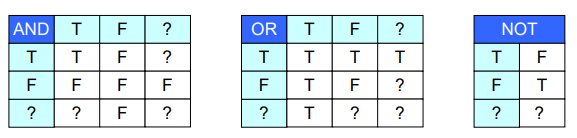
\includegraphics[width=0.7\textwidth]{tabella_verit_sql.png}
  \caption{Tabella di verità}
  \label{fig:tabella_verita-SQL}
\end{figure}
Per valutare gli attributi nulli è necessario usare IS NULL o IS NOT NULL.\\
\begin{itemize}
  \item IS NULL - vero se attributo ha valore nullo, falso altrimenti
  \item IS NOT NULL - vero se attributo ha valore specificato, falso altrimenti
\end{itemize}
\paragraph*{Esempio per la seguente tabella}
\begin{tabular}{|c|c|c|}
  \hline
  A & B & C \\
  \hline
  a & ? & c1 \\
  \hline
  a1 & b & c2 \\
  \hline
  a2 & ? & ? \\
  \hline
\end{tabular}
\begin{lstlisting}[language=SQL]
  SELECT *
  FROM Tabella
  WHERE B IS NULL
\end{lstlisting}
Restituisce t1 e t3.
\paragraph*{Esempio reali} Query: gli impiegati che \textbf{sono} o \textbf{potrebbero essere}
ingegneri.
\begin{lstlisting}[language=SQL]
  SELECT *
  FROM Impiegato
  WHERE mansione = 'Ingegnere' OR mansione IS NULL
\end{lstlisting}
\subsection{SELECT - DISTINCT}
In algebra relazionale i risultati della interrogazioni non contengono
elementi duplicati, mentre in SQL le tabelle prodotte dalle interrogazioni
possono contenere più righe identiche tra loro.\\
I duplicati possono essere rimossi usando la parola chiave DISTINCT.
\begin{lstlisting}[language=SQL]
  SELECT [DISTINCT] AttrEspr
  FROM Tabella
  [WHERE Condizione]
\end{lstlisting}
\subsection{Espressioni e Funzioni}
I predicati usati nelle interrogazioni possono coinvolgere, oltre a
nomi di colonna anche espressioni. Le espressioni sono formulate
applicando operatori ai valori delle colonne delle tuple.\\
Esempi di espressioni e funzioni sono que40lle aritmetiche su stringhe,
su date e tempi. Le espressioni possono comparire nelle clausole
SELECT, WHERE e UPDATE.
\paragraph*{SELECT} Una espressione usata nella clausola SELECT
dà luogo ad una nuova colonna che non corrisponde a nessuna colonna
della tabella su cui si effettua la selezione (argomento di FROM).\\
Questa colonna è detta Colonna \textbf{virtuale}. Le colonne virtuali non sono
fisicamente memorizzate, ma sono materializzate (esistono) solo come risultato
delle interrogazioni.\\
Anche alle colonne virtuali è possibile assegnare un alias (con il
costrutto AS).\\
\paragraph*{Funzioni predefinite}
\begin{itemize}
  \item su stringhe (UPPER, UCASE, LENGTH)
  \item su date, intervalli (+, -, DATE, DAYOFWEEK, ...)
  \item matematiche (*, +, -, /, TAN, SQRT, SIN, ...)
  \item informazioni di istema (USER, CURRENT\_DATE, ...) 
\end{itemize}
\paragraph*{Esempio} Trovare stipendio mensile degli impiegati che guadagnano
più di 40.\\
Dato che lo stipendio memorizzato nel DB è annuale, bisogna dividere per 12.
\begin{lstlisting}[language=SQL]
  SELECT stipendio/12 AS stipendio_mensile
  FROM Impiegato
  WHERE stipendio > 40
\end{lstlisting}
Se non inserisco un ALIAS la colonna virtuale avrà un nome generato (non significativo).
\paragraph*{Funzioni per le stringhe}
Gli operatori più comuni sono:
\begin{itemize}
  \item || - concatenazione
  \item UPPER, UCASE - Trasforma la stringa in caratteri maiuscoli
  \item LOWER, LCASE - Trasforma la stringa in caratteri minuscoli
\end{itemize}

